\scanpage{89}
$X$, topos\\
$k$ Anneau sur $X$

$k\overset{u}{\hookrightarrow}\Phi$ mono dans $k$-Module, avec
\[
\left\{\begin{array}{ll}
\text{\textcircled{a}}&\Psi=\operatorname{Coker}u\quad k\text{-plat}\\
\text{\textcircled{b}}&\forall\ k\text{-modules }M,N,\text{ et }i>0\\
&\Gamma^i(N\otimes_k\Phi)\otimes M\longrightarrow\text{flasque}
\end{array}\right.
\]

\uline{Lemme} $\forall$ $k$-modules $\unsure{S|B}$, $\exists$ \deleted{hom} $S\overset{u_S}{\longrightarrow}\unsure{\widetilde N|\overleftarrow N}$, qui \textcircled{a} est un $k$-mono ``universel'' (reste mono par tensorisation) tel que $\unsure{S|N}$ plat $\Rightarrow$ $\operatorname{Coker}\unsure{u_N|u_S}$ plat, et \textcircled{b'} $\forall i>0$, et $k$ modules $\unsure{N|P},M$
\[
\Gamma_k^i(\widetilde N\otimes_k P)\otimes_k M\quad\text{flasque}
\]

\margin{\figure{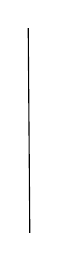
\begin{tikzpicture}\draw (0,0)--(.02,-2.6);\end{tikzpicture}}}

On prend $\widetilde N=\unsure{\Phi}\otimes_k\unsure{S|B}$, $u_S=u\otimes\operatorname{id}_S$, d'où a) résulte de a), et b') de b).

\[
\mathcal{DR}_{pd}^{**}(\deleted{\unsure{k,\Phi}}k,u)
=\Gamma^*(\Psi)\otimes_k\Lambda^*\Psi
\]
Anneau bigradué (degré compl. + degré ext. = degré total)
\inserted{alterné pour deg. ext.}
différentiel à p.d. (sur idéal des \unsure{bidegrés} $>0\unsure{\ldots}$) une résolution de $k\{T\}$. (où deg ext $T=0$, deg tot $T=1$)
\[
\mathrm{DR}_{pd}^{**}(k,u)=\Gamma(X,\mathcal{DR}_{pd}^{**}(k,u)).
\]

Soit $\mathbb{DR}^{**}$ la cat \inserted{\uline{dérivée}} des anneaux bigradués (à deg $\geq0$) alternés diff. à p.d., \inserted{avec \unsure{un $T$ élémt marqué} pur bidegré $(1,0)$} on \unsure{définit} un syst. transitif d'isom. dans $\mathbb{DR}^{**}$ entre les $\mathrm{DR}_{pd}^{**}(k,u)$, pour $k$ fixé et $u$ variable.

Notons que si on a
\diagram{\begin{tikzcd}
&\Phi \arrow[dd,"\lambda"]\\
k \arrow[ur,"u"] \arrow[dr,"u'"',dash]&\\
&\Phi'
\end{tikzcd}}
d'où
$\lambda^{**}:\mathrm{DR}_{pd}^{**}(k,u)\mathbin{-}\mathrm{DR}_{pd}^{**}(k,u')$,
donc $\lambda^{**}$ est un iso. dans $\mathbb{DR}^{**}$.

\unsure{\diagram{\begin{tikzcd}
&\Phi' \arrow[dr,hook]& &\\
k \arrow[ur,hook,"u"] \arrow[dr,hook,"u'"']&&S \arrow[r,hook,"\text{donné par lemme}"] \arrow[d,equal]&N\\
&\Phi \arrow[ur,hook] &\Phi\amalg_k\Phi'&
\end{tikzcd}}}

d'où
\diagram{\begin{tikzcd}
\mathrm{DR}(u)\arrow[dr,"\sim"]&\\
&\mathrm{DR}(N)\\
\mathrm{DR}(u')\arrow[ur,"\sim"]&
\end{tikzcd}}
d'où $\mathrm{DR}(u)\simeq\unsure{\mathrm{DR}(u')}$ dans $\mathbb{DR}^{**}$

indépendant du choix de $S\hookrightarrow N$ avec $N$ comme dans le lemme
\unsure{\diagram{\begin{tikzcd}
&N \arrow[dr,hook]&&\\
S \arrow[ur,hook] \arrow[dr,hook]&&T \arrow[r,hook,"\text{donné par lemme}"]\arrow[d,equal]&N''\\
&N' \arrow[ur,hook]&N\amalg_S N'&
\end{tikzcd}}}
\margin{$k$}
d'où
\diagram{\begin{tikzcd}
\mathrm{DR}(u)\arrow[dr]&&\mathrm{DR}(N)\arrow[dr,"\sim"]&\\
&\mathrm{DR}(S)\arrow[ur]\arrow[dr]&&\mathrm{DR}(N''\qquad\sim\\
\mathrm{DR}(u')\arrow[ur]&&\mathrm{DR}(N')\arrow[ur,"\sim"]&
\end{tikzcd}}

Transitivité évidente par \unsure{diagramme}.

\margin{88}
